\chapter{Anforderungsanalyse und Methodik}
\label{cha:anforderungsanalyse}

In der klassischen Ausprägung des Wasserfallmodells stellt die Anforderungsanalyse (Requirements Engineering) die fundamentale erste Projektphase dar. Gemäß dieser Methodik müssen alle funktionalen und nicht-funktionalen Anforderungen sowie Hardware- und Software-Restriktionen zu Beginn der Entwicklung definiert werden. Das Ziel ist es, eine verlässliche und überprüfbare Basis für die nachfolgenden Phasen (Design, Implementierung und Validierung) zu schaffen, um spätere Planungsänderungen zu vermeiden.

\section{Hardware- und Softwareanforderungen}
Aus der übergeordneten Systemauslegung des Bierkühlers wurden spezifische Anforderungen an die Software und die Elektronik abgeleitet. Die nachfolgende Tabelle (Tab.~\ref{tab:all_requirements}) listet die zentralen technischen Anforderungen auf, die für die Umsetzung der Steuerung relevant sind.

\begin{table}[h]
	\centering
	\caption{Vollständige Anforderungsliste des Projekts (Mechanik, Elektronik \& Software)}
	\label{tab:all_requirements}
	\begin{tabularx}{\textwidth}{l X c}
		\toprule
		\textbf{ID} & \textbf{Anforderung (Beschreibung)} & \textbf{Typ} \\
		\midrule
		ID-0001 & In den Bierkühler müssen verschiedene Flaschengrößen (0,33 L und 0,5 L) passen. & Design \\
		\addlinespace
		ID-0002 & Gleiche Trinktemperatur (4 bis 7°C) bei jeder initialen Flaschentemperatur. & Performance \\
		\addlinespace
		ID-0003 & Das Bier darf sich nicht zu schnell drehen, um übermäßiges Schäumen zu verhindern. & Performance \\
		\addlinespace
		ID-0004 & Das Bier darf beim Drehen nicht durchrutschen (Sicherstellung des mechanischen Kontakts). & Funktional \\
		\addlinespace
		ID-0005 & Das Eis soll im laufenden Betrieb unkompliziert wieder auffüllbar sein. & Design \\
		\addlinespace
		ID-0006 & Der Behälter muss vollständig wasserdicht sein. & Funktional \\
		\addlinespace
		ID-0007 & Es soll eine feste Skala für den Füllstand des Wassers/Eises geben (Min/Max). & Design \\
		\addlinespace
		ID-0008 & Die Software muss zwei Temperatursensoren über ADC-Kanäle auslesen und in Echtzeit verarbeiten. & Funktional \\
		\addlinespace
		ID-0010 & Die Software muss Eingaben vom Drehregler über ADC oder EXTI-Interrupt erfassen und interpretieren. & Funktional \\
		\addlinespace
		ID-0011 & Die Software muss das LCD-Display über I²C ansteuern und die aktuellen Temperaturen anzeigen. & Funktional \\
		\addlinespace
		ID-0013 & Die Software muss PWM-Signale generieren, um Pumpe und Motor stufenlos zu steuern (ersetzt das ursprünglich geplante Relais). & Funktional \\
		\addlinespace
		ID-0014 & Die Software muss DMA-Unterstützung für das effiziente ADC-Sampling der Sensoren nutzen. & Performance \\
		\addlinespace
		ID-0015 & Die Spannungswandlung von 12V auf 3,3V muss berücksichtigt und stabile Betriebsbedingungen für die MCU sichergestellt werden. & Design \\
		\addlinespace
		ID-0016 & Die Software muss eine Fehlerbehandlung für die ADC-Kanäle implementieren. & Funktional \\
		\bottomrule
	\end{tabularx}
\end{table}

\section{Anforderungsdefinition im Wasserfall-Modell}
Da wir uns in diesem Projekt für einen Ablauf nach dem klassischen Wasserfall-Modell entschieden haben, war es zwingend notwendig, die Anforderungen zu Beginn der Entwicklungsphase zu fixieren. Hierbei gaben die mechanischen Restriktionen und das übergeordnete Projektmanagement (insbesondere die strikte Kosteneffizienz für eine potenzielle Serienproduktion) den Rahmen für die elektronischen Anforderungen vor.

Um strukturierte und verifizierbare Ziele zu formulieren, wurden die Anforderungen nach dem SMART-Prinzip definiert und in funktionale Anforderungen (z. B. Temperaturmessung) sowie Performance- und Design-Anforderungen unterteilt. Ein wesentliches Merkmal unserer angewandten Methodik ist dabei die sogenannte Traceability: Jede in Tabelle~\ref{tab:all_requirements} definierte ID dient als direkte Vorgabe für die spätere Testspezifikation und Validierungsphase.

\subsection{Technical Trade-offs und Hardware-Limitierungen}
Obwohl das Wasserfall-Modell systematische Änderungen im Nachhinein erschwert, zwangen uns physische Limitierungen bei der Evaluation der Hardware zu einem kritischen \textit{Technical Trade-off}. Ursprünglich war ein binäres Schalten von Pumpe und Motor über ein elektromechanisches Relais angedacht. Bei der Konzeption stellte sich jedoch heraus, dass die GPIO-Pins des aus Kostengründen gewählten Mikrocontrollers STM32F030C8T6 nicht ausreichend Leistung bereitstellen konnten, um ein Relais direkt oder stabil über einfache Treiberstufen anzusteuern.

Um dieses Hardware-Limit zu lösen und gleichzeitig die Systemanforderung an einen schaumfreien Kühlprozess (ID-0003) zu erfüllen, wurde die Vorgabe ID-0013 angepasst: Die Relais-Steuerung wurde durch eine PWM-basierte Ansteuerung (Pulsweitenmodulation) über Leistungs-MOSFETs ersetzt. Diese Design-Entscheidung entlastete den Mikrocontroller elektrisch und ermöglichte erst die präzise, stufenlose Regelung der Motordrehzahl, die für die Erfüllung der mechanischen Performance-Ziele zwingend notwendig war. Diese Anpassung wurde sauber dokumentiert und floss als feste Basis in die nachfolgende Implementierungsphase ein.

\begin{figure}[h]
	\centering
	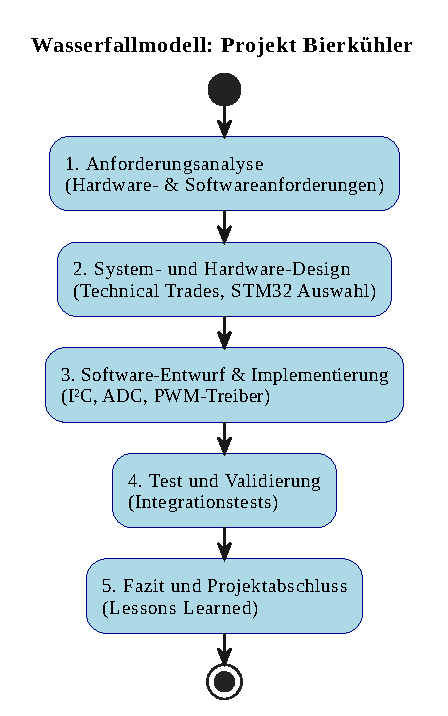
\includegraphics[width=0.5\textwidth]{images/wasserfallmodel.pdf} 
	\caption{Phasenablauf des Projekts nach dem Wasserfallmodell}
	\label{fig:wasserfall}
\end{figure}

Das Projektziel fokussierte auf eine kosteneffiziente Entwicklung, die eine spätere Serienproduktion ermöglicht. Aus diesem Grund wurde bei der Komponentenauswahl ein striktes Kostenmanagement verfolgt, welches beispielsweise zur Wahl des Mikrocontrollers STM32-F030C8T6 führte. Im Rahmen des gewählten Wasserfall-Modells wurden alle benötigten Komponenten frühzeitig identifiziert und beschafft. Verzögerungen in der Testphase, bedingt durch Lieferzeiten und personelle Engpässe in der frühen Projektphase, wurden als Risiko identifiziert und durch eine straffe Planung in der anschließenden Implementierungsphase kompensiert. Deswegen ist auch die Anzahl der Anforderungen / Requirements mit dem Projekt nicht wirklich gewachsen oder wurde nennenswert verändert. 
